\newif\ifimagen\imagentrue
\documentclass[11pt]{article}
\usepackage{fullpage}\usepackage{mathptmx}\usepackage{latexsym}\usepackage{graphicx}\usepackage{amsmath, amssymb, amsthm, amsfonts}\usepackage{algpseudocode}\newcommand{\handout}[5]{
   \renewcommand{\thepage}{#1-\arabic{page}}
   \noindent
   \begin{center}
   \framebox{
      \vbox{
    \hbox to 5.78in { {\bf COMPSCI 634: Geometric Algorithms} \hfill #2 }
       \vspace{4mm}
       \hbox to 5.78in { {\Large \hfill #5  \hfill} }
       \vspace{2mm}
       \hbox to 5.78in { {\it #3 \hfill #4} }
      }
   }
   \end{center}
   \vspace*{4mm}
}
\renewcommand{\paragraph}[1]{\medskip \noindent {\bf #1.}}
\newcommand{\lecture}[4]{\handout{#1}{#2}{Lecturer: #3}{Scribe: #4}{Lecture #1}}
\newtheorem{definition}{Definition}
\newtheorem{algorithm}{Algorithm}
\newtheorem{openquestion}{Open Question}
\newtheorem{remark}{Remark}
\newtheorem{theorem}{Theorem}
\newtheorem{lemma}[theorem]{Lemma}
\newtheorem{corollary}[theorem]{Corollary}
\newtheorem{fact}[theorem]{Fact}
\newcommand{\example}[1]{\paragraph{Example #1}}

\pagestyle{empty}
\thispagestyle{empty}
\begin{document}
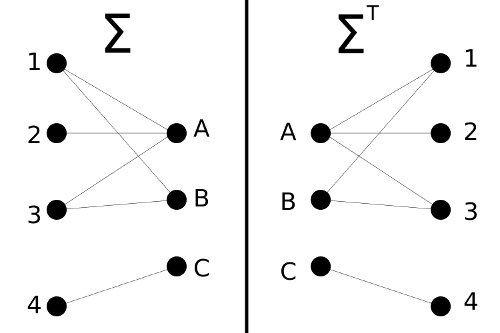
\includegraphics[width=0.4\textwidth]{./BipartiteGraph.png}
\clearpage% page: 0
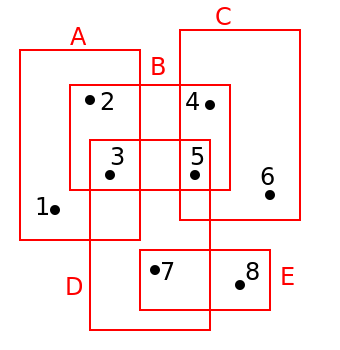
\includegraphics[width=0.5\textwidth]{./RectanglePoints.png}
\clearpage% page: 1
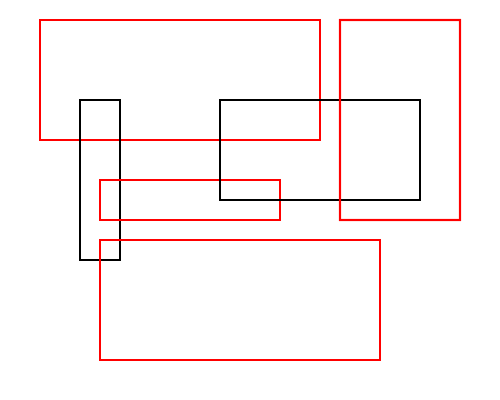
\includegraphics[width=0.5\textwidth]{./RectangleIndySet.png}
\clearpage% page: 2
%Options: 
\end{document}
